\section{Statistical Analysis}

\textbf{Data Collection}

\textit{Population vs Sample}


\begin{center}
	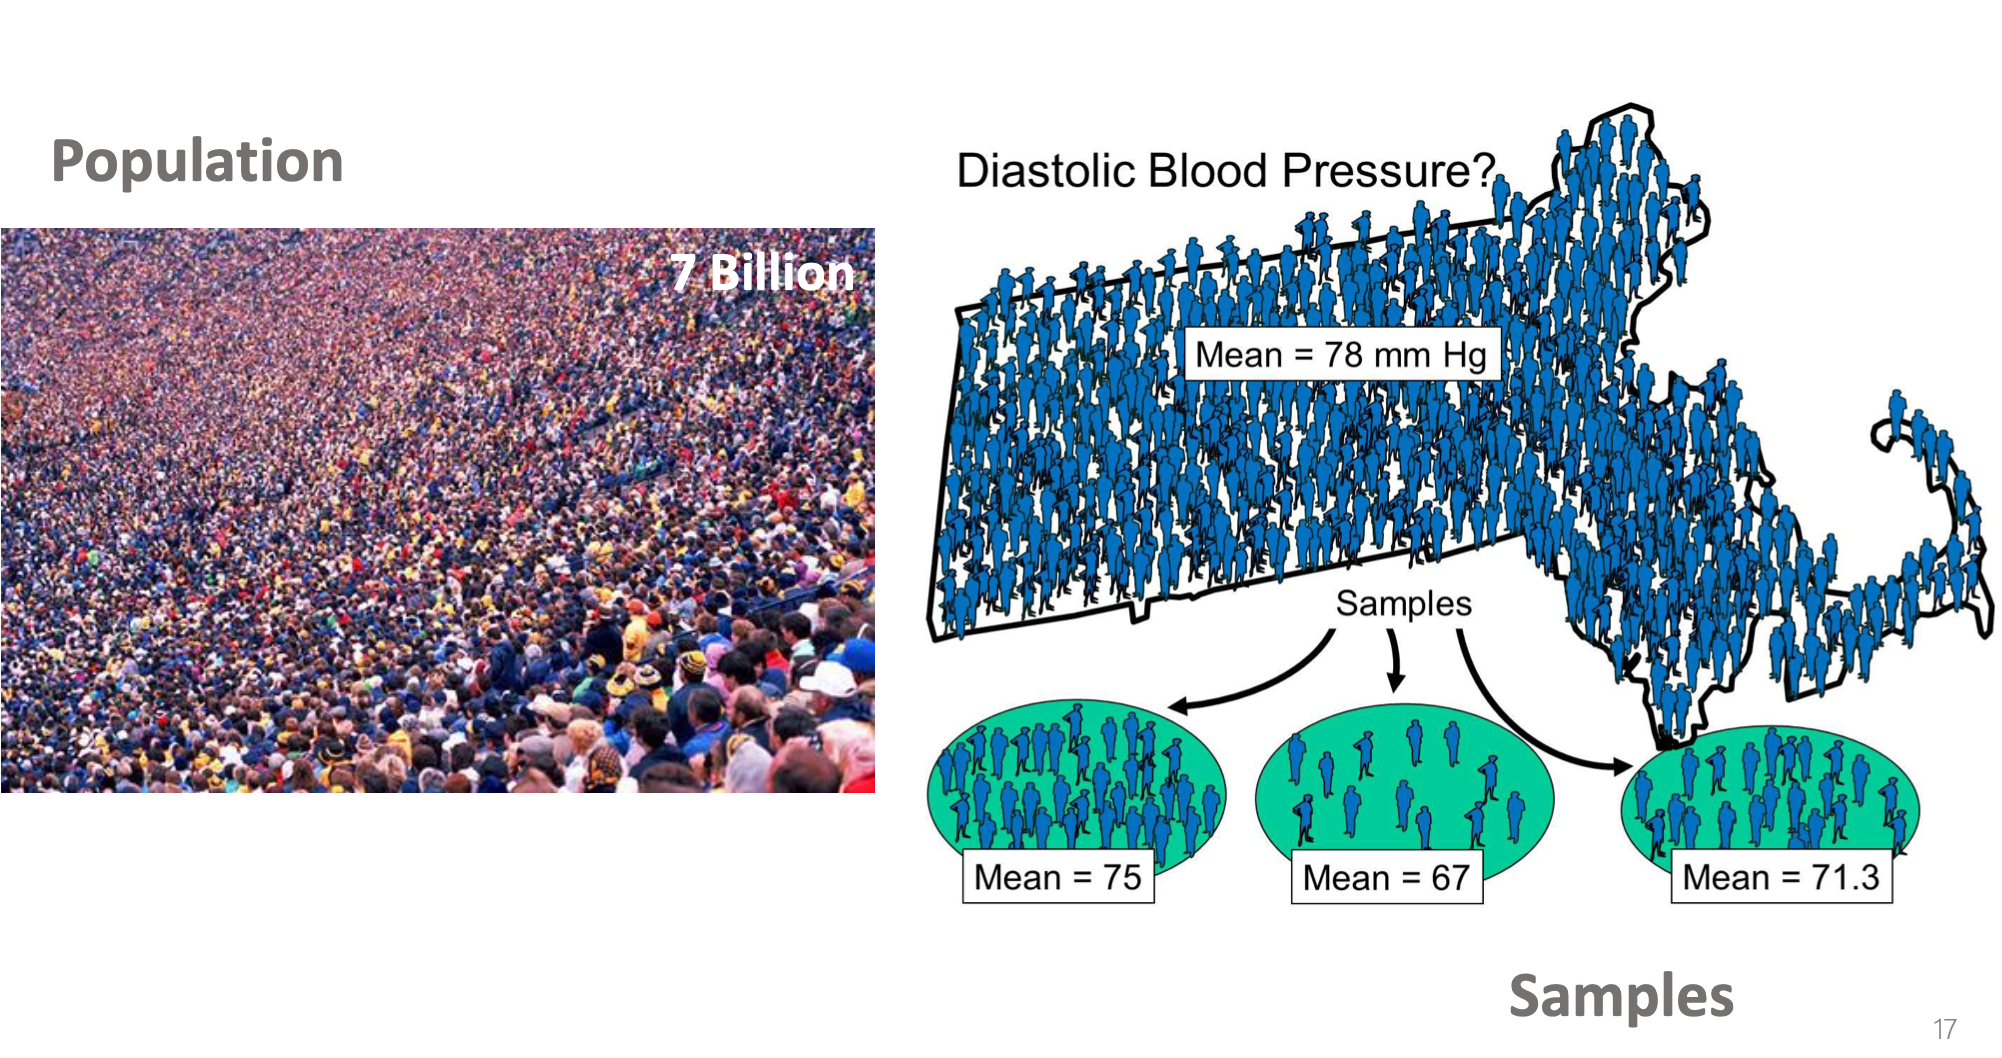
\includegraphics[width=\linewidth]{population_sample.png}
\end{center}


\textit{Generalizability}


\textit{Hypothesis testing}


\textbf{Descriptive statistics and validation}

\textit{Mean}

\textit{Median}


\textit{Distribution}

\textit{Confidence Interval (CI)}


\textbf{Analysis}

\textit{Frequentist Approaches}


\textit{Hypothesis testing}

\textit{P-Value}

\textit{Alpha-Level}

\textit{Errors}

\textit{Degrees of Freedom}


\textit{Independent vs dependent samples}


\textit{Parametrix vs. non-parametric tests}


\textit{A/B Testing}


\textit{Indepdendent t-test}


\textit{From t-value to significance}


\textit{ANOVA analysis of Variance}


\textit{Effect size}

\textit{Powere analysis}


\textit{Software for statistical analysis}


\textbf{Reporting}


\textit{Writing up the results}













